% Options for packages loaded elsewhere
\PassOptionsToPackage{unicode}{hyperref}
\PassOptionsToPackage{hyphens}{url}
\PassOptionsToPackage{dvipsnames,svgnames,x11names}{xcolor}
%
\documentclass[
  12pt,
]{article}
\usepackage{amsmath,amssymb}
\usepackage{iftex}
\ifPDFTeX
  \usepackage[T1]{fontenc}
  \usepackage[utf8]{inputenc}
  \usepackage{textcomp} % provide euro and other symbols
\else % if luatex or xetex
  \usepackage{unicode-math} % this also loads fontspec
  \defaultfontfeatures{Scale=MatchLowercase}
  \defaultfontfeatures[\rmfamily]{Ligatures=TeX,Scale=1}
\fi
\usepackage{lmodern}
\ifPDFTeX\else
  % xetex/luatex font selection
\fi
% Use upquote if available, for straight quotes in verbatim environments
\IfFileExists{upquote.sty}{\usepackage{upquote}}{}
\IfFileExists{microtype.sty}{% use microtype if available
  \usepackage[]{microtype}
  \UseMicrotypeSet[protrusion]{basicmath} % disable protrusion for tt fonts
}{}
\makeatletter
\@ifundefined{KOMAClassName}{% if non-KOMA class
  \IfFileExists{parskip.sty}{%
    \usepackage{parskip}
  }{% else
    \setlength{\parindent}{0pt}
    \setlength{\parskip}{6pt plus 2pt minus 1pt}}
}{% if KOMA class
  \KOMAoptions{parskip=half}}
\makeatother
\usepackage{xcolor}
\usepackage[margin=1in]{geometry}
\usepackage{longtable,booktabs,array}
\usepackage{calc} % for calculating minipage widths
% Correct order of tables after \paragraph or \subparagraph
\usepackage{etoolbox}
\makeatletter
\patchcmd\longtable{\par}{\if@noskipsec\mbox{}\fi\par}{}{}
\makeatother
% Allow footnotes in longtable head/foot
\IfFileExists{footnotehyper.sty}{\usepackage{footnotehyper}}{\usepackage{footnote}}
\makesavenoteenv{longtable}
\usepackage{graphicx}
\makeatletter
\def\maxwidth{\ifdim\Gin@nat@width>\linewidth\linewidth\else\Gin@nat@width\fi}
\def\maxheight{\ifdim\Gin@nat@height>\textheight\textheight\else\Gin@nat@height\fi}
\makeatother
% Scale images if necessary, so that they will not overflow the page
% margins by default, and it is still possible to overwrite the defaults
% using explicit options in \includegraphics[width, height, ...]{}
\setkeys{Gin}{width=\maxwidth,height=\maxheight,keepaspectratio}
% Set default figure placement to htbp
\makeatletter
\def\fps@figure{htbp}
\makeatother
\setlength{\emergencystretch}{3em} % prevent overfull lines
\providecommand{\tightlist}{%
  \setlength{\itemsep}{0pt}\setlength{\parskip}{0pt}}
\setcounter{secnumdepth}{5}
\newlength{\cslhangindent}
\setlength{\cslhangindent}{1.5em}
\newlength{\csllabelwidth}
\setlength{\csllabelwidth}{3em}
\newlength{\cslentryspacingunit} % times entry-spacing
\setlength{\cslentryspacingunit}{\parskip}
\newenvironment{CSLReferences}[2] % #1 hanging-ident, #2 entry spacing
 {% don't indent paragraphs
  \setlength{\parindent}{0pt}
  % turn on hanging indent if param 1 is 1
  \ifodd #1
  \let\oldpar\par
  \def\par{\hangindent=\cslhangindent\oldpar}
  \fi
  % set entry spacing
  \setlength{\parskip}{#2\cslentryspacingunit}
 }%
 {}
\usepackage{calc}
\newcommand{\CSLBlock}[1]{#1\hfill\break}
\newcommand{\CSLLeftMargin}[1]{\parbox[t]{\csllabelwidth}{#1}}
\newcommand{\CSLRightInline}[1]{\parbox[t]{\linewidth - \csllabelwidth}{#1}\break}
\newcommand{\CSLIndent}[1]{\hspace{\cslhangindent}#1}
\usepackage{floatrow}
\floatsetup{capposition=top}
\usepackage{setspace}
\usepackage{fancyhdr}
\usepackage{titlesec}
\usepackage{geometry}
\usepackage{subfig}
\newcommand{\beginsupplement}{
\setcounter{table}{0}
\renewcommand{\thetable}{S\arabic{table}}
\setcounter{figure}{0}
\renewcommand{\thefigure}{S\arabic{figure}}}
\usepackage{booktabs}
\usepackage{longtable}
\usepackage{array}
\usepackage{multirow}
\usepackage{wrapfig}
\usepackage{float}
\usepackage{colortbl}
\usepackage{pdflscape}
\usepackage{tabu}
\usepackage{threeparttable}
\usepackage{threeparttablex}
\usepackage[normalem]{ulem}
\usepackage{makecell}
\usepackage{xcolor}
\ifLuaTeX
  \usepackage{selnolig}  % disable illegal ligatures
\fi
\IfFileExists{bookmark.sty}{\usepackage{bookmark}}{\usepackage{hyperref}}
\IfFileExists{xurl.sty}{\usepackage{xurl}}{} % add URL line breaks if available
\urlstyle{same}
\hypersetup{
  pdftitle={A Sociological Analysis of Structural Racism in `Student List' Lead Generation Products},
  pdfauthor={Ozan Jaquette; Karina G. Salazar},
  colorlinks=true,
  linkcolor={Maroon},
  filecolor={Maroon},
  citecolor={Blue},
  urlcolor={blue},
  pdfcreator={LaTeX via pandoc}}


\begin{document}


\newpage

\hypertarget{tables}{%
\section{Tables}\label{tables}}

\begin{table}[!h]

\caption{\label{tab:orders-filters-combo}Top filter combinations used in College Board orders purchased purchased by research vs. master's}
\centering
\resizebox{\linewidth}{!}{
\begin{tabular}[t]{lcclcc}
\toprule
\multicolumn{3}{c}{\textbf{Research}} & \multicolumn{3}{c}{\textbf{M.A.}} \\
\cmidrule(l{3pt}r{3pt}){1-3} \cmidrule(l{3pt}r{3pt}){4-6}
\textbf{Filters} & \textbf{Count} & \textbf{Percent} & \textbf{Filters} & \textbf{Count} & \textbf{Percent}\\
\midrule
HS grad class, GPA, SAT, Zip code & 99 & 19\% & HS grad class, GPA, PSAT, Zip code & 143 & 47\%\\
HS grad class, GPA, SAT, PSAT, Rank, State, Race & 39 & 7\% & HS grad class, GPA, SAT, Zip code & 107 & 35\%\\
HS grad class, SAT, State & 38 & 7\% & HS grad class, GPA, SAT, PSAT, Zip code & 28 & 9\%\\
HS grad class, PSAT, State & 28 & 5\% & HS grad class, SAT, Geomarket & 6 & 2\%\\
HS grad class, GPA, SAT, State & 23 & 4\% & HS grad class, GPA, SAT, PSAT, County & 4 & 1\%\\
\addlinespace
HS grad class, GPA, PSAT, State, Race & 20 & 4\% & HS grad class, GPA, SAT, County & 4 & 1\%\\
HS grad class, PSAT, State, Low SES & 20 & 4\% & HS grad class, SAT, Geomarket, College type & 2 & 1\%\\
HS grad class, GPA, PSAT, State & 19 & 4\% & HS grad class, PSAT, Geomarket & 2 & 1\%\\
HS grad class, GPA, AP score, Geomarket & 15 & 3\% & HS grad class, GPA, SAT, State, Segment, Major, Edu aspiration & 1 & 0\%\\
HS grad class, GPA, SAT, PSAT, State, Segment, Gender & 13 & 2\% & HS grad class, GPA, PSAT, State, Geomarket, Edu aspiration & 1 & 0\%\\
\bottomrule
\end{tabular}}
\end{table}

\begingroup\fontsize{8}{12}\selectfont

\emph{NOTES: Top filter combinations are based on 830 College Board student list purchases made by research (N=9) and master's (N=5) universities from 2016-2020. Geodemographic and Segment filters are proprietary filters created by College Board that use geodemography to predict the college-going behaviors of students within specific geographic areas.}

\clearpage

\newpage

\hypertarget{figures}{%
\section{Figures}\label{figures}}

\begin{figure}

{\centering 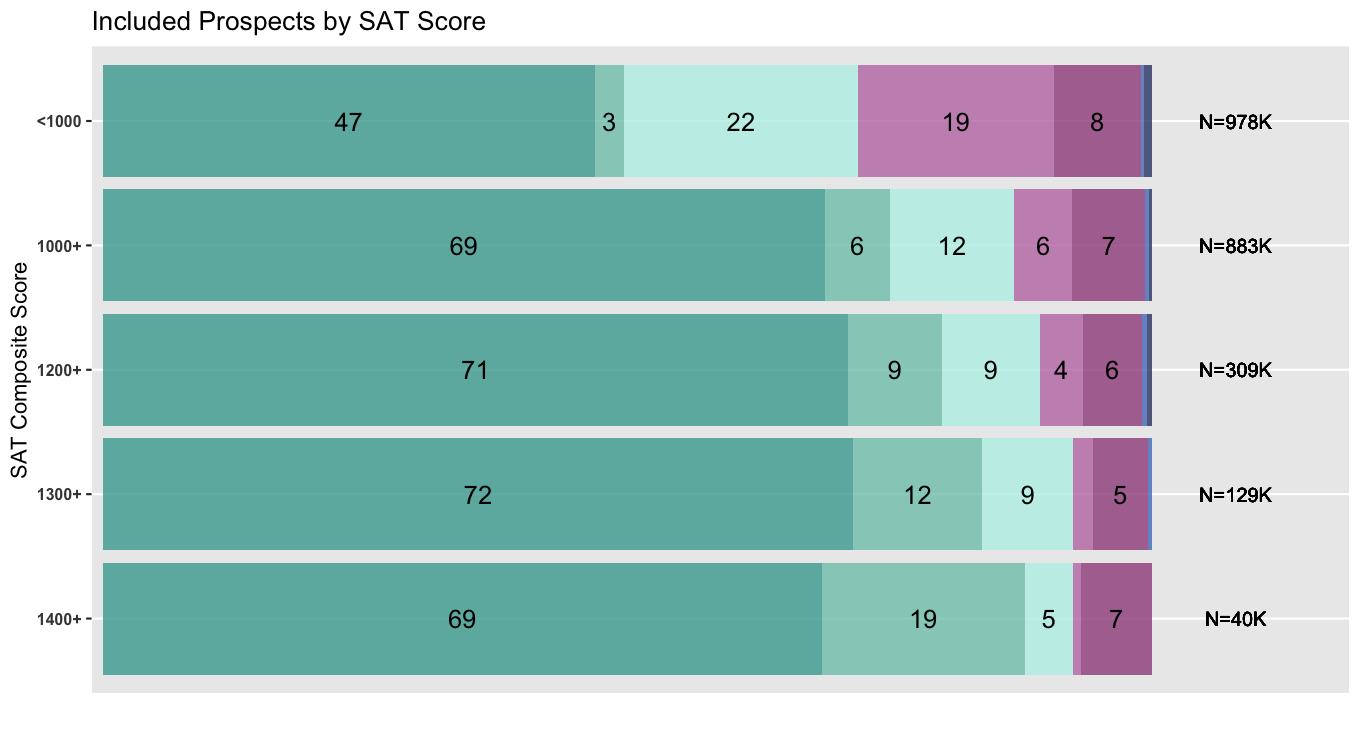
\includegraphics[width=0.35\linewidth]{./../../outputs/figures/p2_sat_incv2} 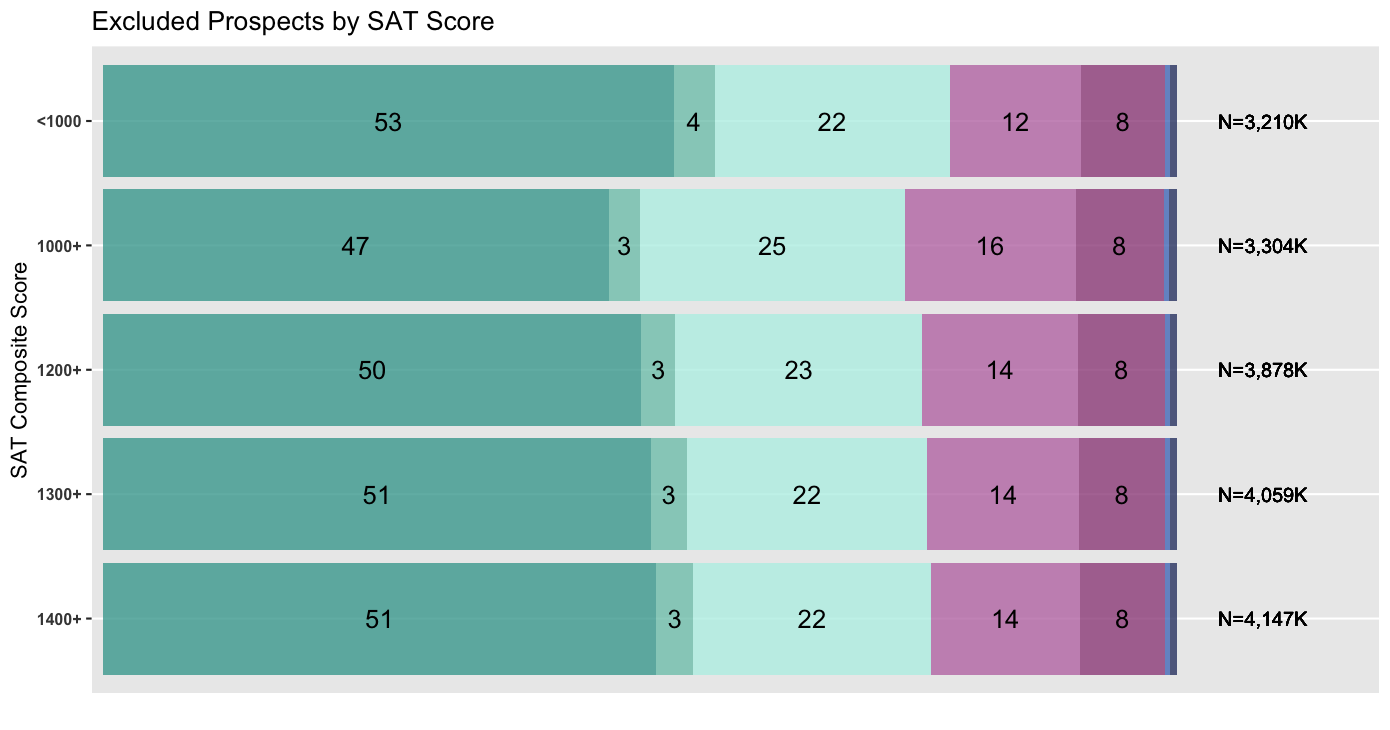
\includegraphics[width=0.35\linewidth]{./../../outputs/figures/p2_sat_excv2} 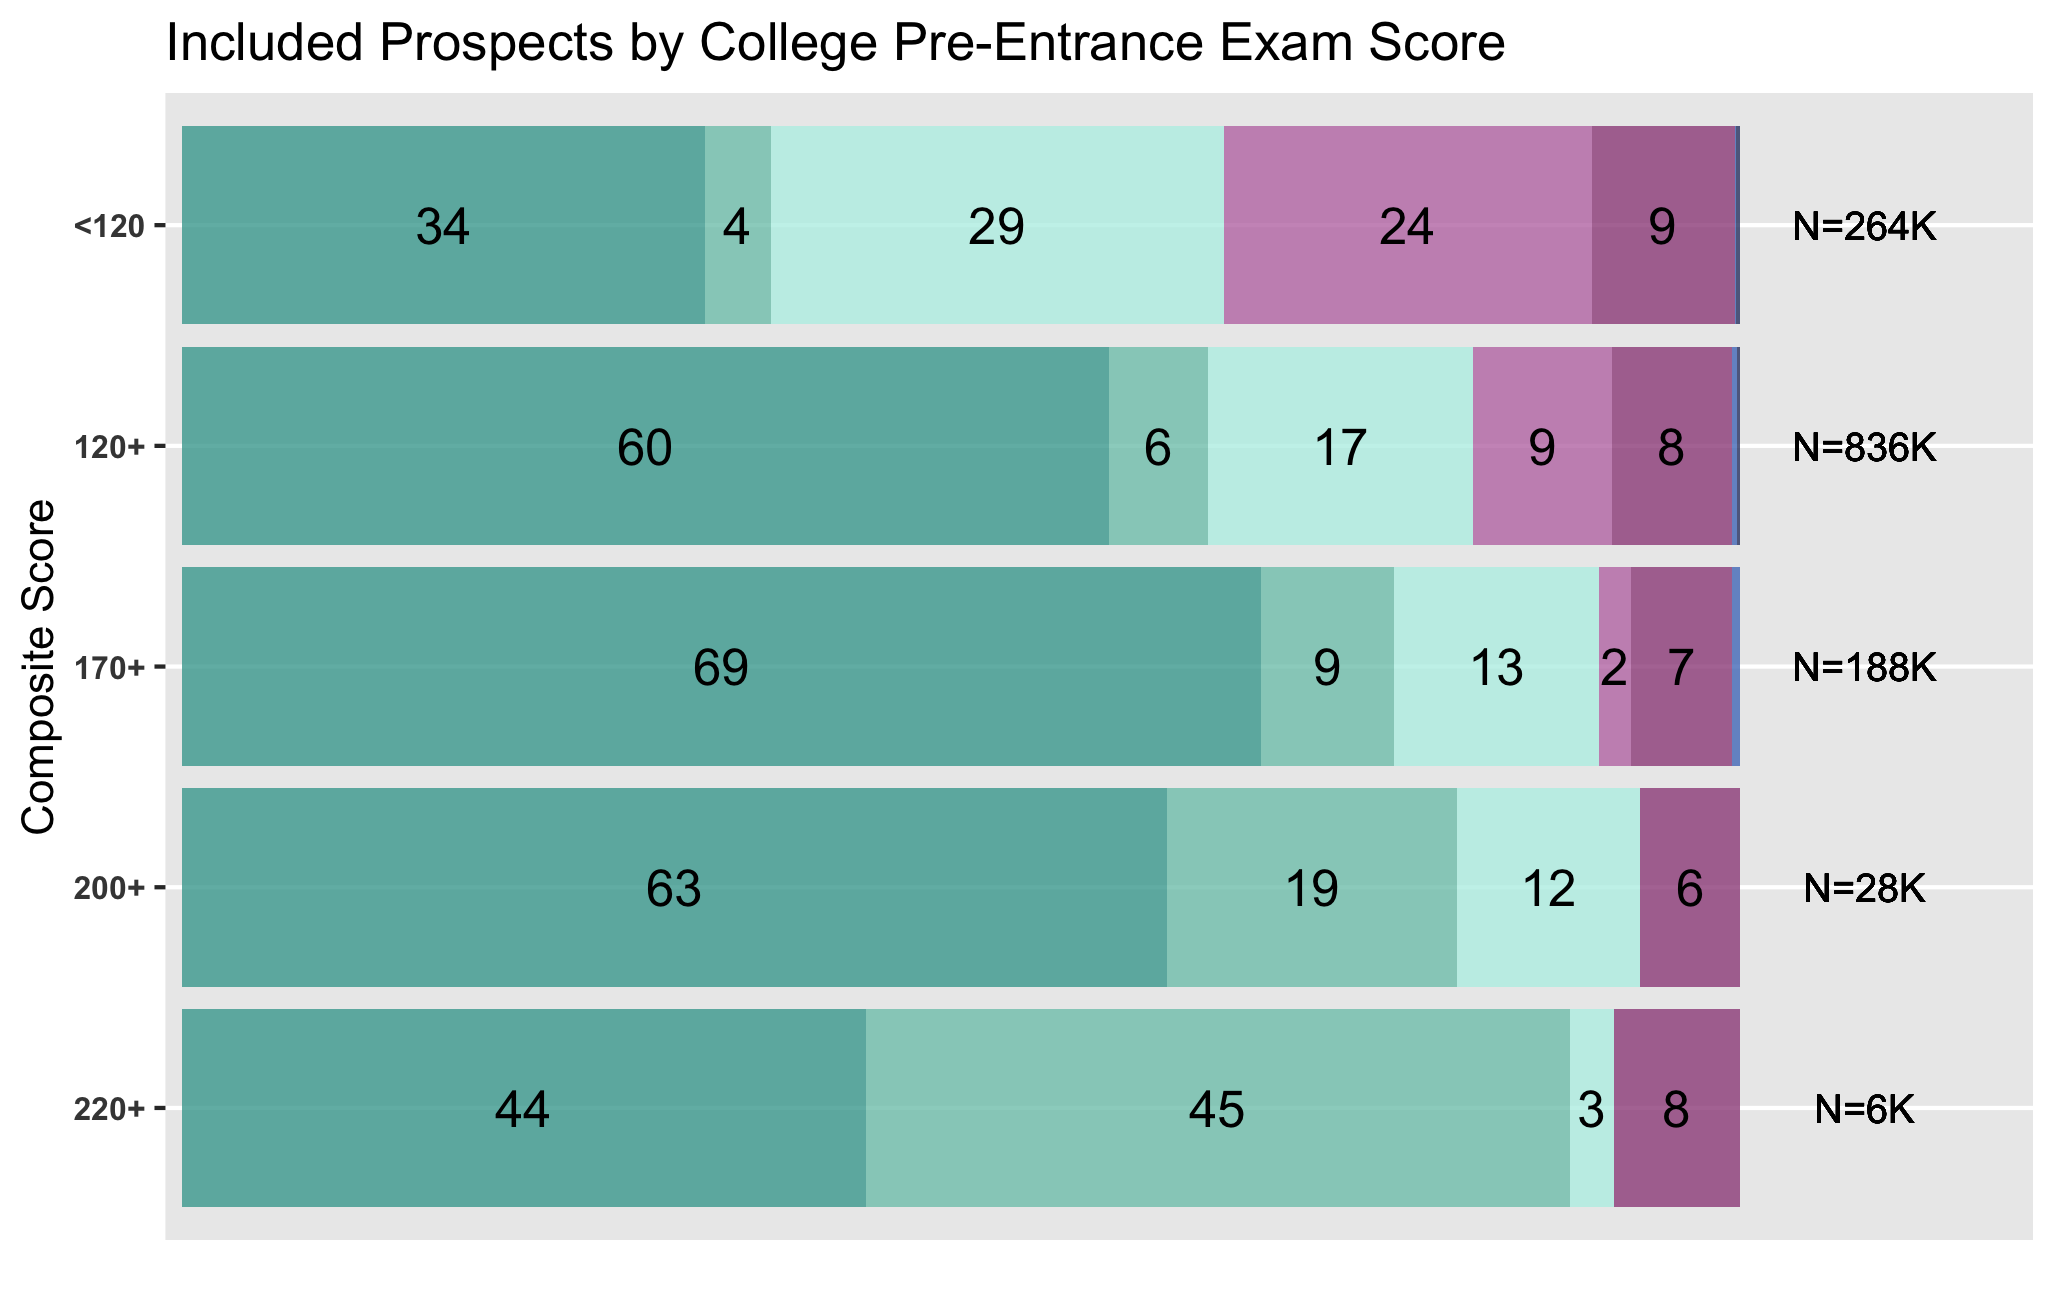
\includegraphics[width=0.35\linewidth]{./../../outputs/figures/p2_psat_incv2} 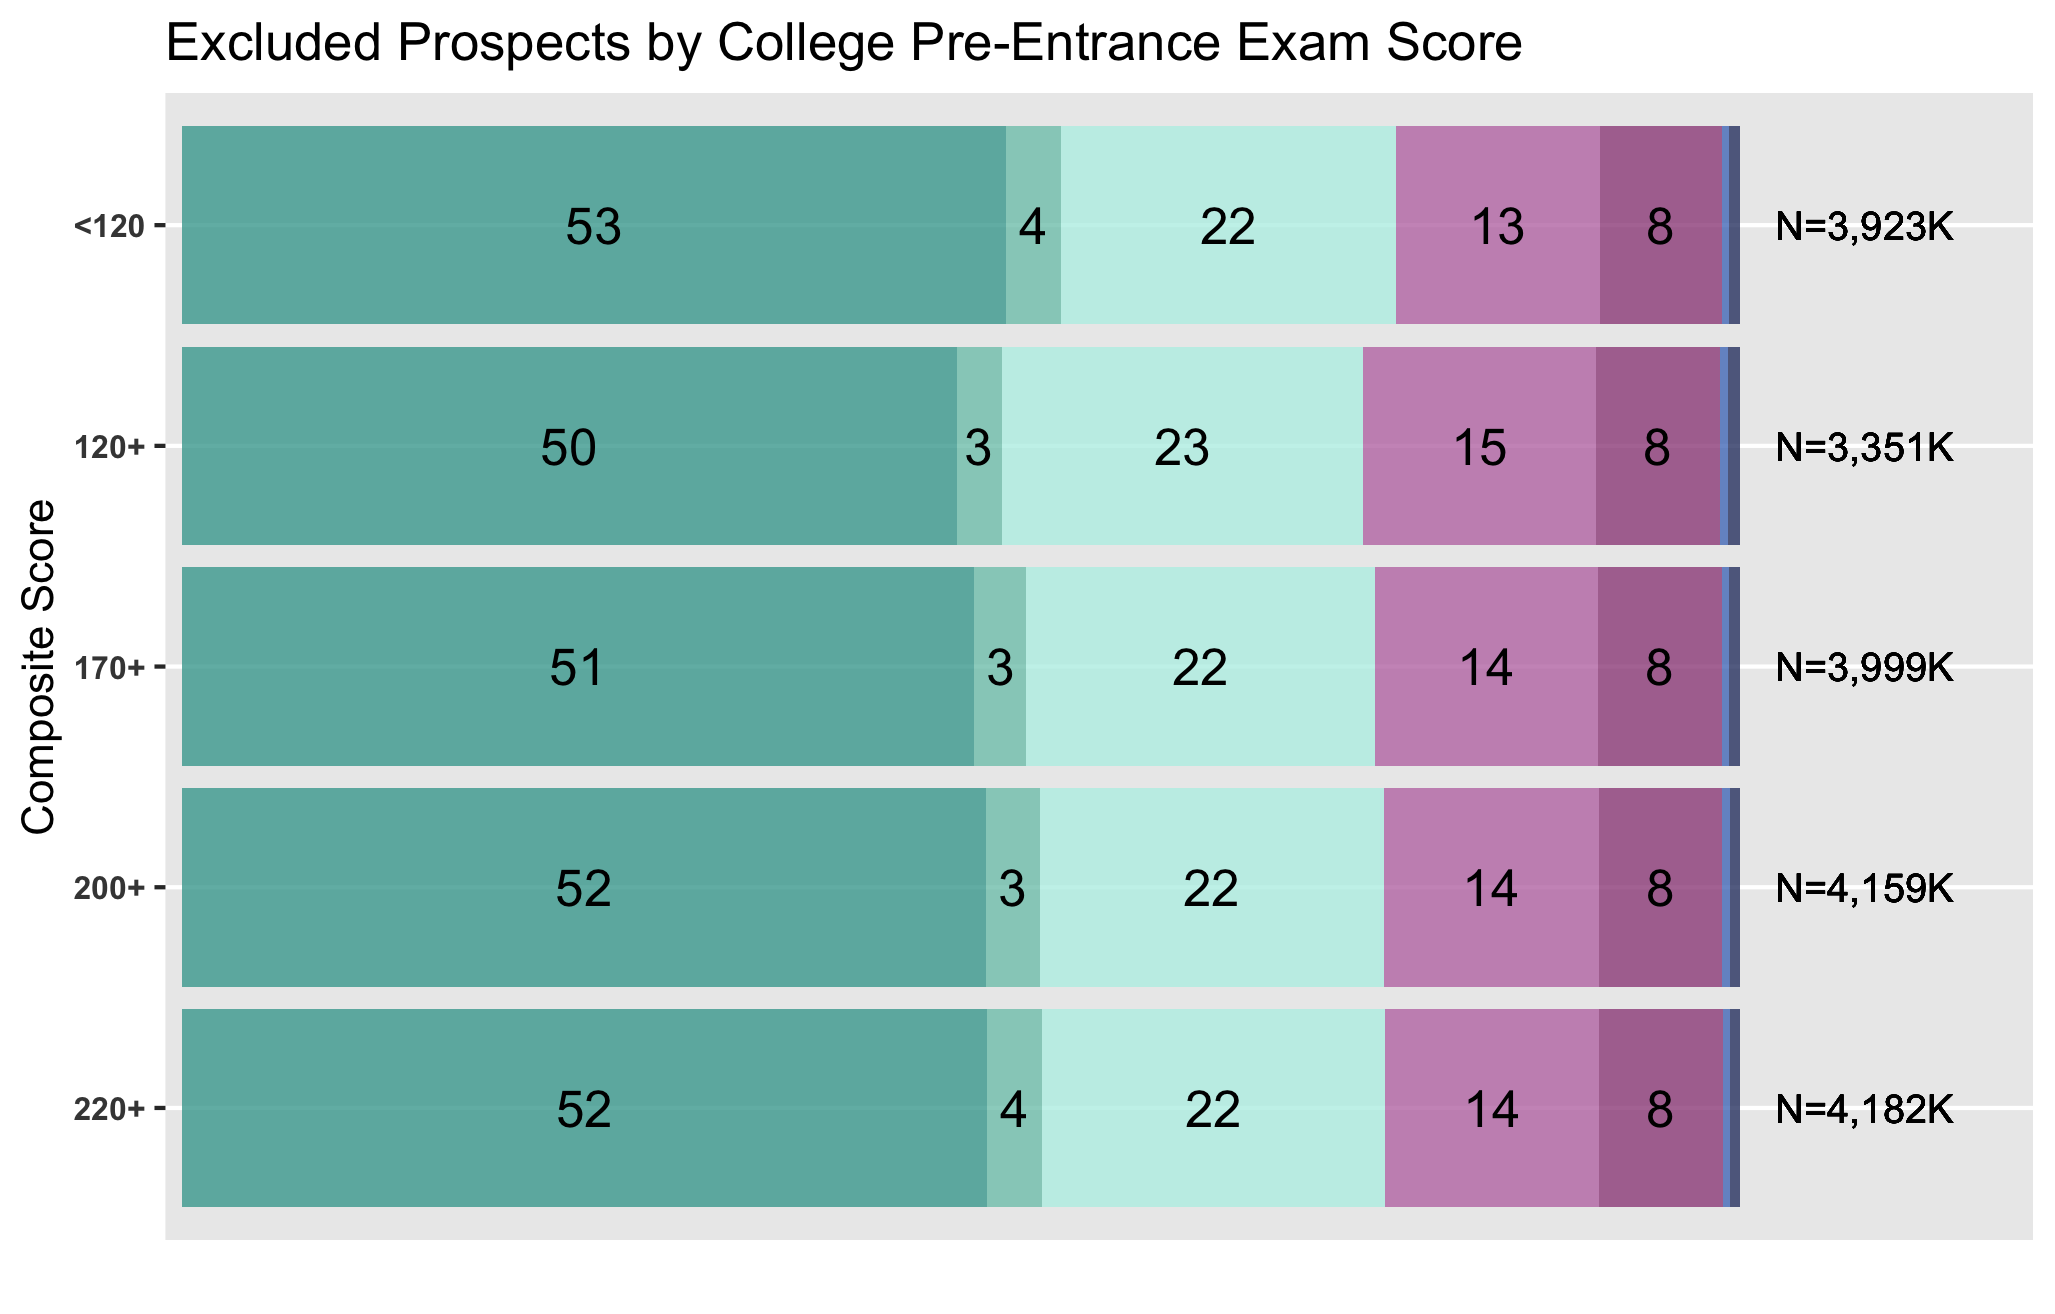
\includegraphics[width=0.35\linewidth]{./../../outputs/figures/p2_psat_excv2} 
\includegraphics[width=0.35\linewidth]{./../../outputs/figures/legend_horizontal} 

}

\caption{College Entrance and Pre-Entrance Exam Filters Across Thresholds}\label{fig:thresholds-tests}
\end{figure}

\begingroup
\fontsize{8}{8}\selectfont

SOURCE: U.S. Department of Education, National Center for Education Statistics, High School Longitudinal Study of 2009 (HSLS09).
\endgroup

\begin{figure}

{\centering 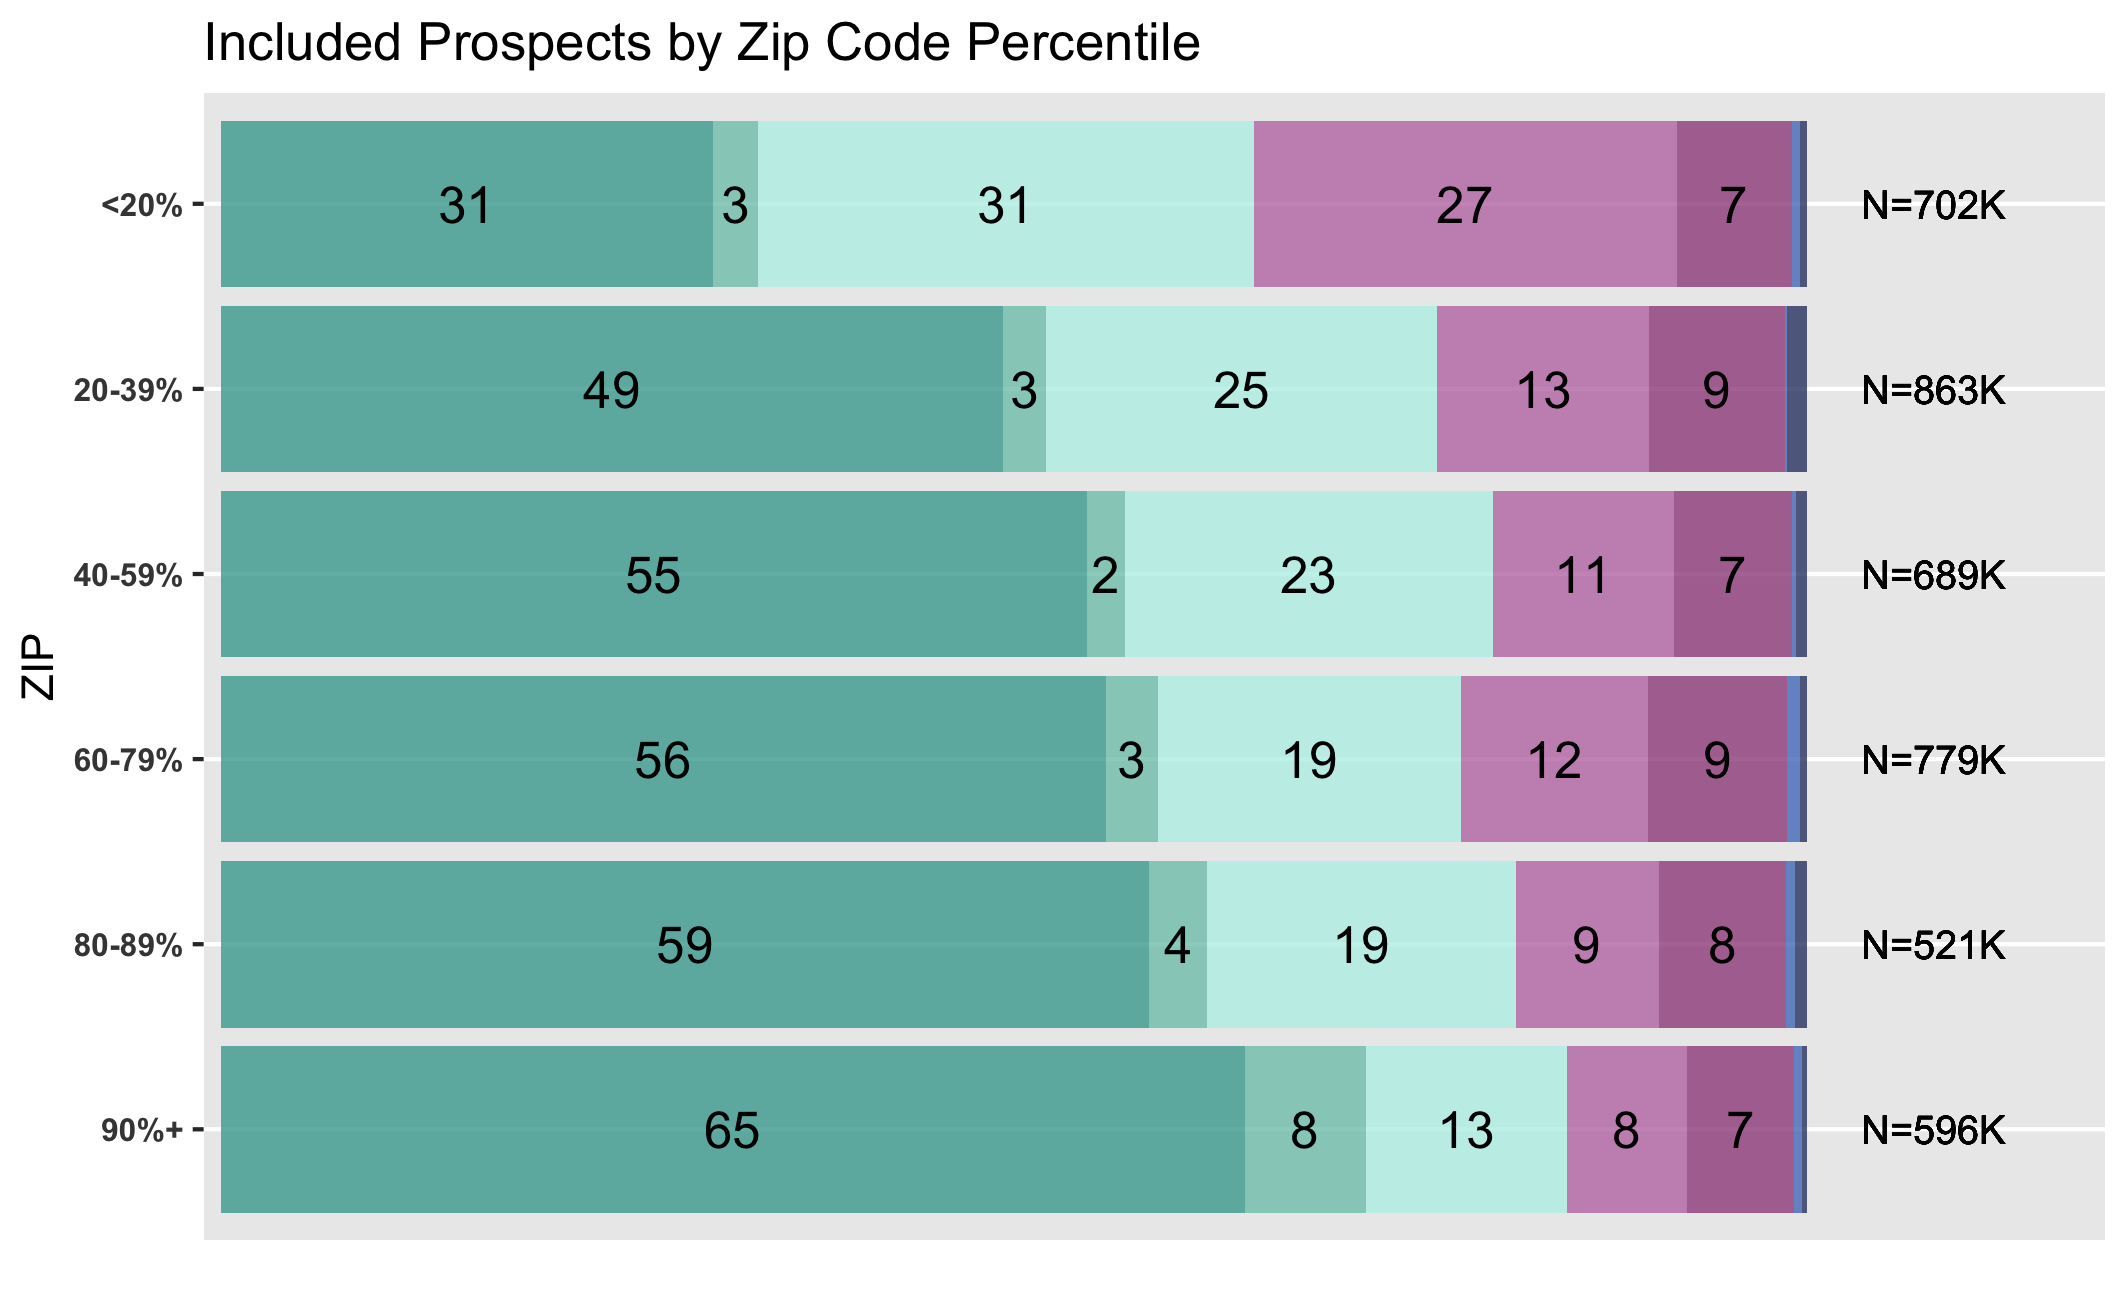
\includegraphics[width=0.4\linewidth]{./../../outputs/figures/p3_zip_incV2} 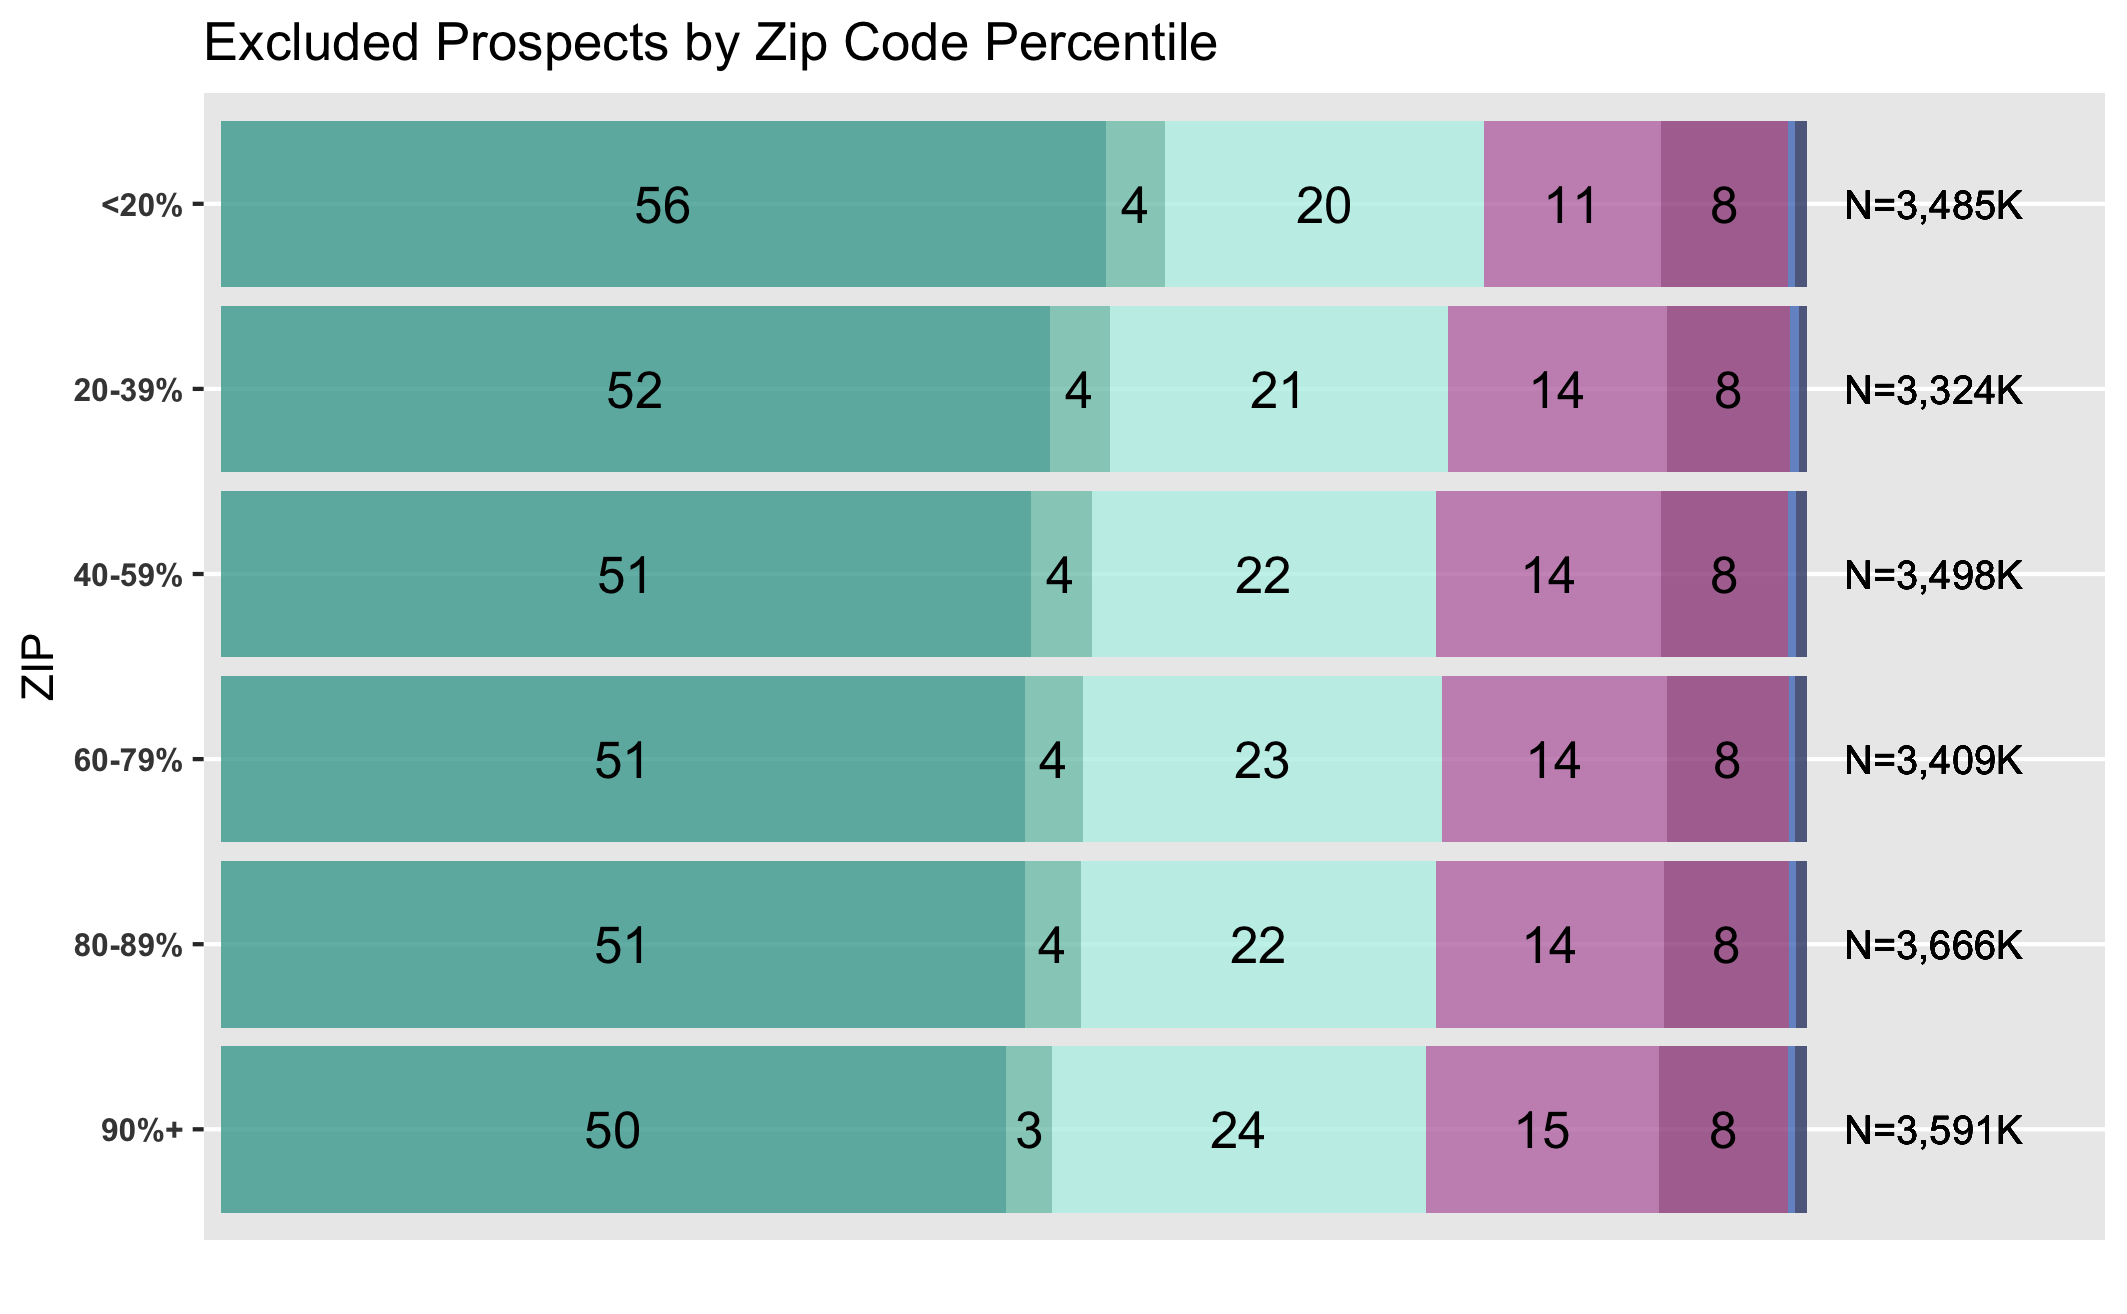
\includegraphics[width=0.4\linewidth]{./../../outputs/figures/p3_zip_excV2} 
\includegraphics[width=0.4\linewidth]{./../../outputs/figures/legend_horizontal} 

}

\caption{Zip Code Filter Across Affluence Percentiles}\label{fig:zipcode-affluence}
\end{figure}

\begingroup
\fontsize{8}{8}\selectfont

SOURCE: U.S. Department of Education, National Center for Education Statistics, High School Longitudinal Study of 2009 (HSLS09).
\endgroup

\textbackslash end\{landscape\}
\pagebreak
\restoregeometry

\begin{figure}
\centering
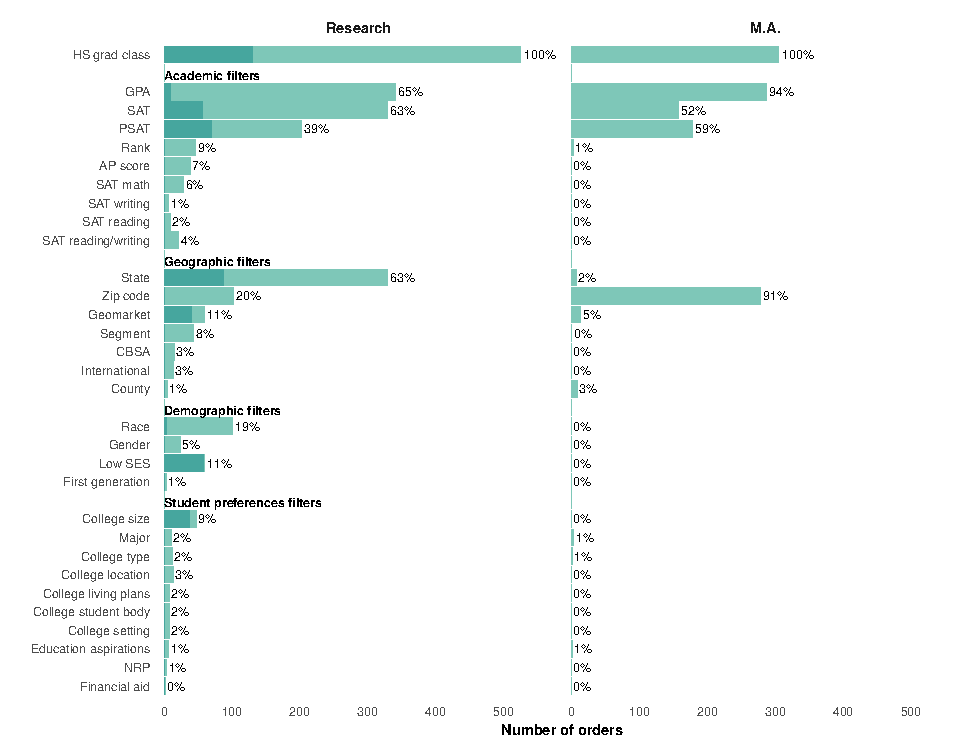
\includegraphics{eepa_student_list_manuscript_c_a_files/figure-latex/order-filters-empirical-report-1.pdf}
\caption{\label{fig:order-filters-empirical-report}Filters used in College Board Orders Purchased by 14 Public Universities}
\end{figure}

\begingroup
\fontsize{8}{8}\selectfont

NOTE: One research university placed a large amount of orders, which influenced the overall filters used for all research universities. The contribution of this particular university is shown in the darker color in the figure.
\endgroup

\begin{figure}
\centering
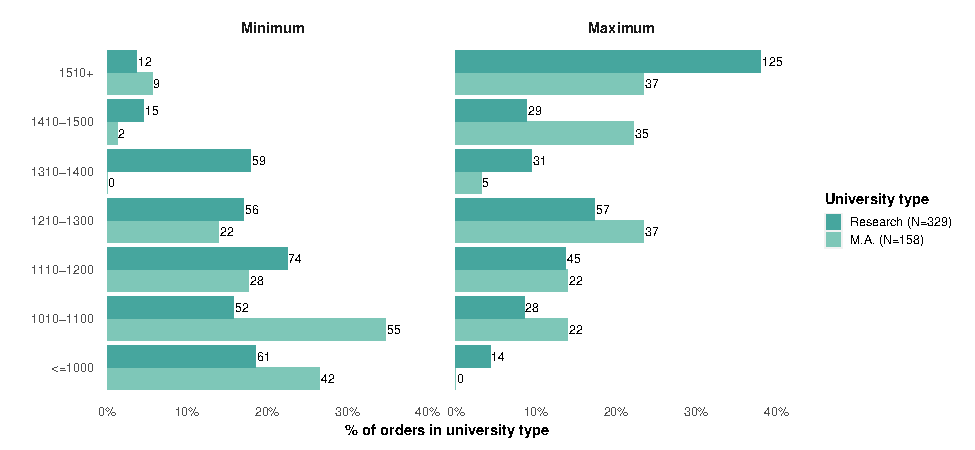
\includegraphics{eepa_student_list_manuscript_c_a_files/figure-latex/orders-sat-1.pdf}
\caption{\label{fig:orders-sat}SAT Filter Used by Research vs.~Master's Public Universities}
\end{figure}

\pagebreak

\begin{landscape}



\begin{figure}

{\centering 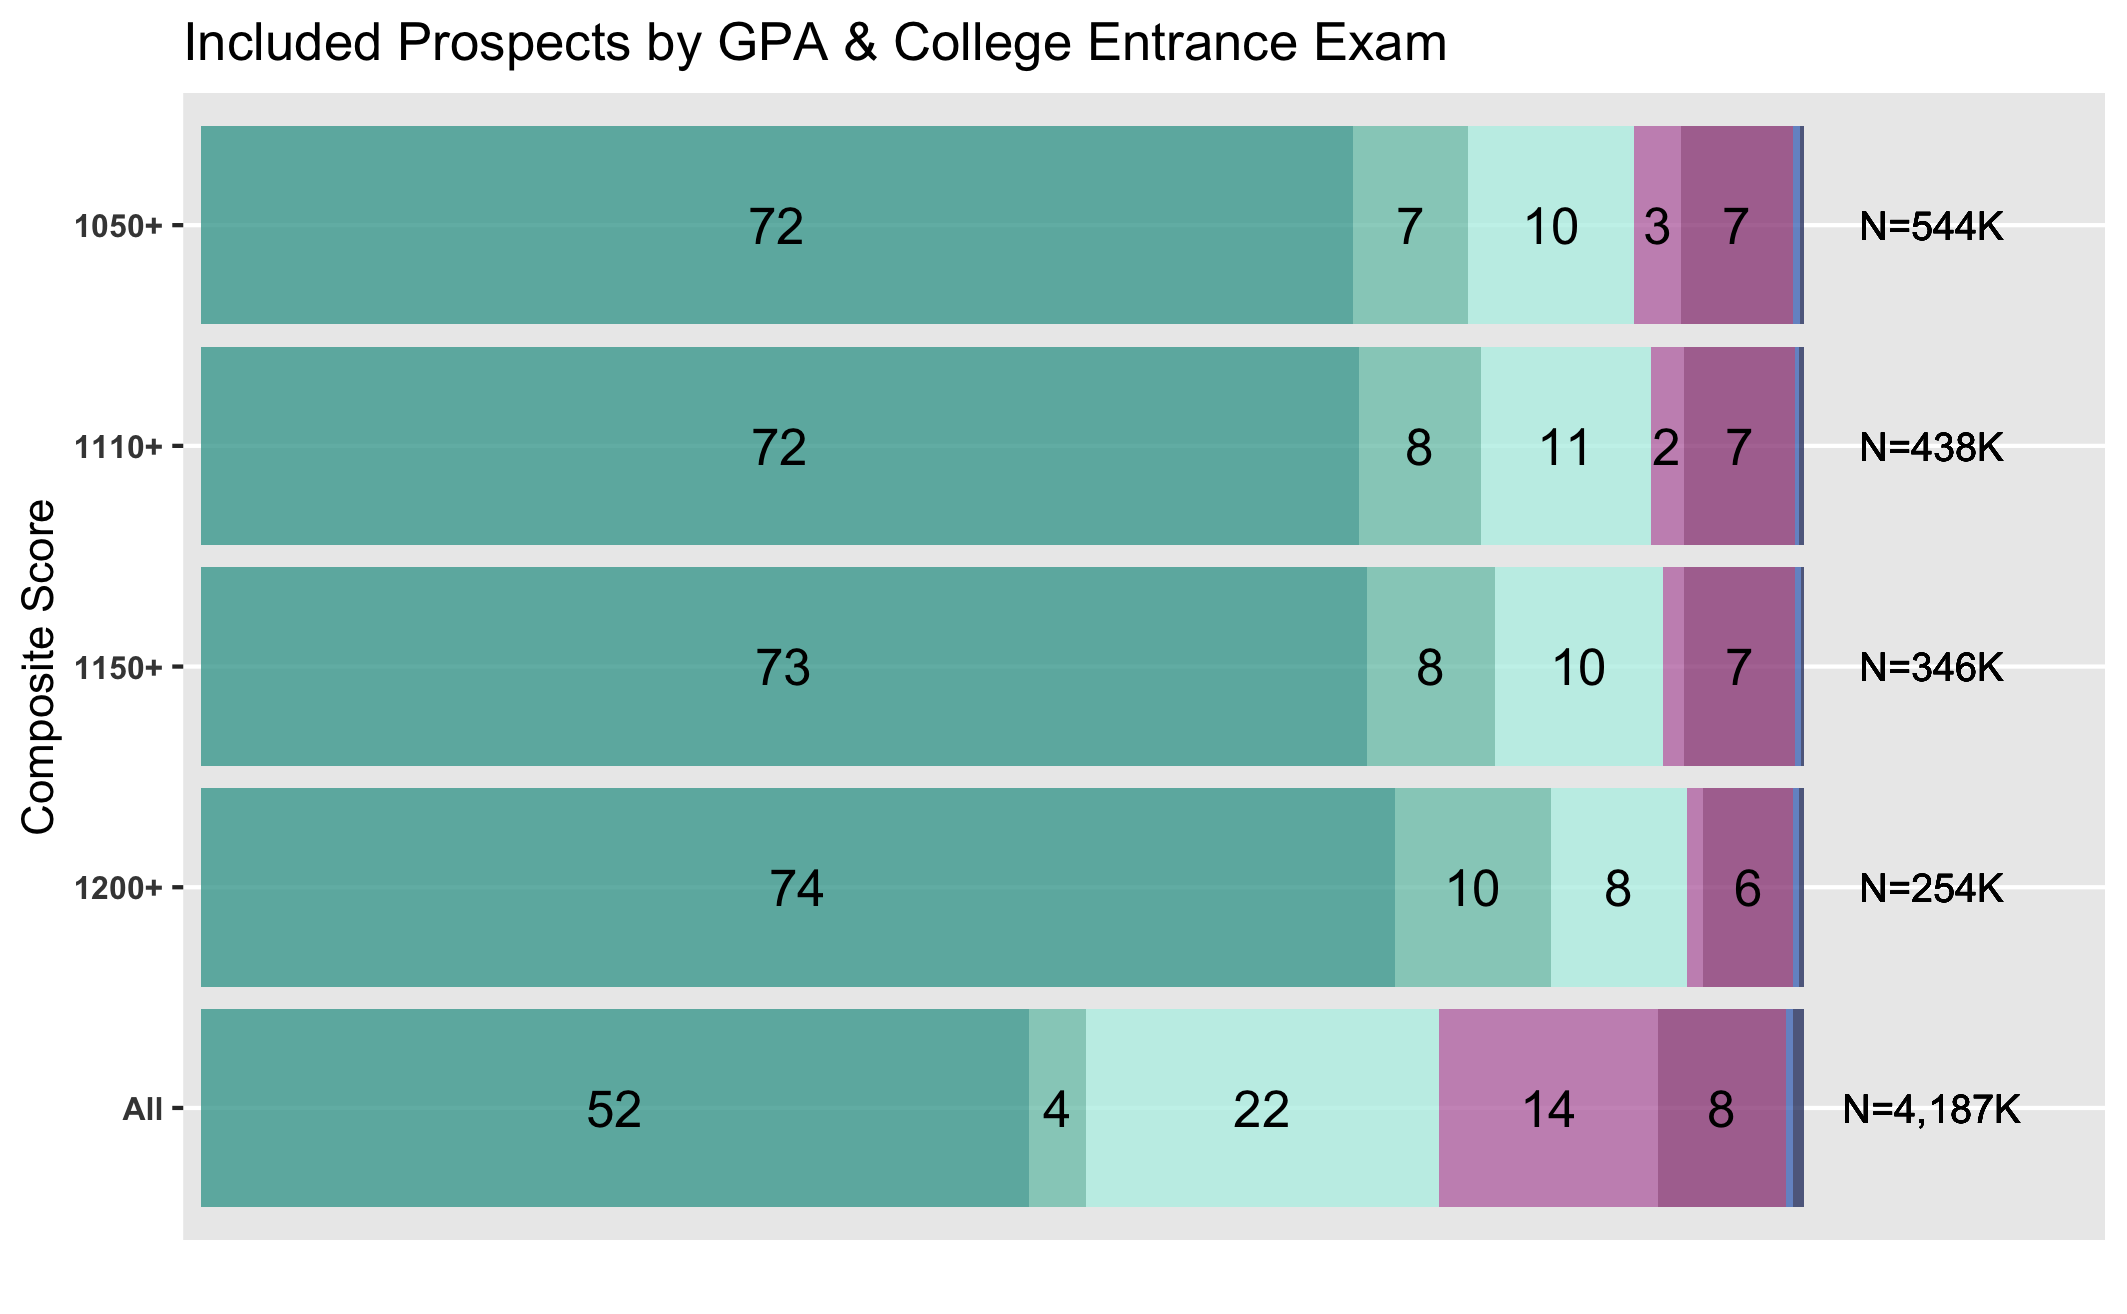
\includegraphics[width=3in]{./../../outputs/figures/combo1_inc_satv2} 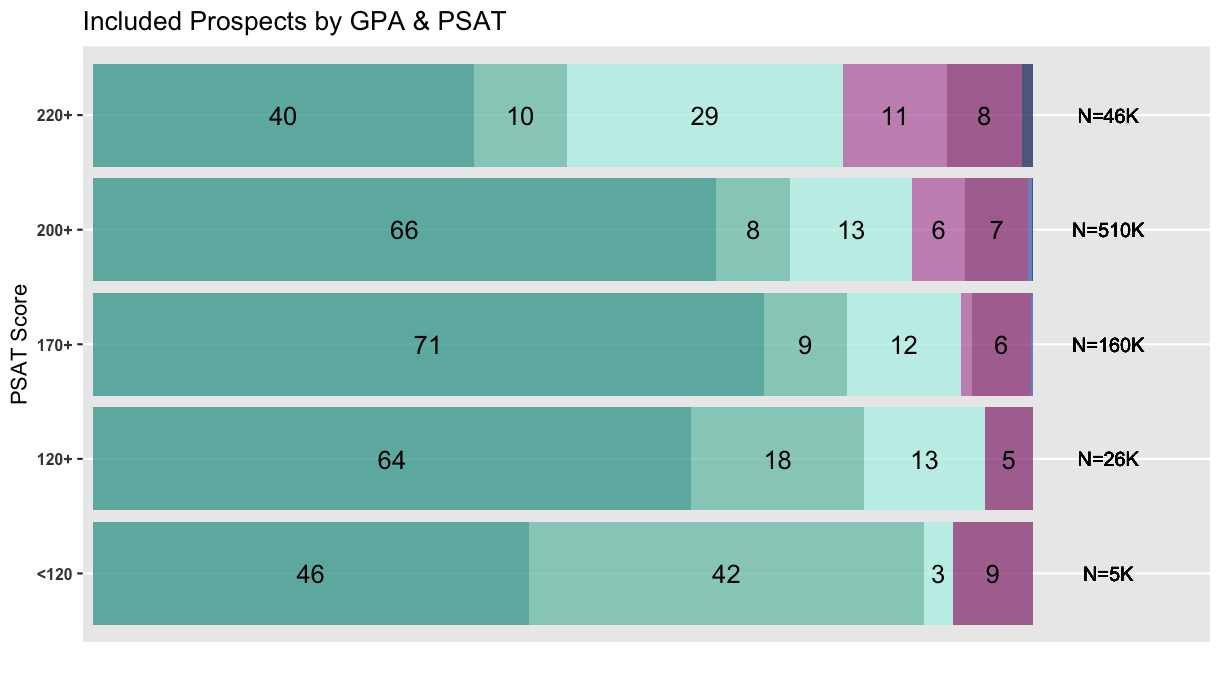
\includegraphics[width=3in]{./../../outputs/figures/combo1_inc_psatv2} 

}

\caption{Academic Combinations: GPA (3.0+) and College Entrance or Pre-Entrance Exams (across score thresholds)}\label{fig:gpa-sat-psat}
\end{figure}


\begin{center}
\includegraphics[width=0.32\linewidth]{./../../outputs/figures/legend_horizontal} \end{center}

\begingroup
\fontsize{8}{8}\selectfont
SOURCE: U.S. Department of Education, National Center for Education Statistics, High School Longitudinal Study of 2009 (HSLS09).
\endgroup

\pagebreak


\begin{figure}

{\centering 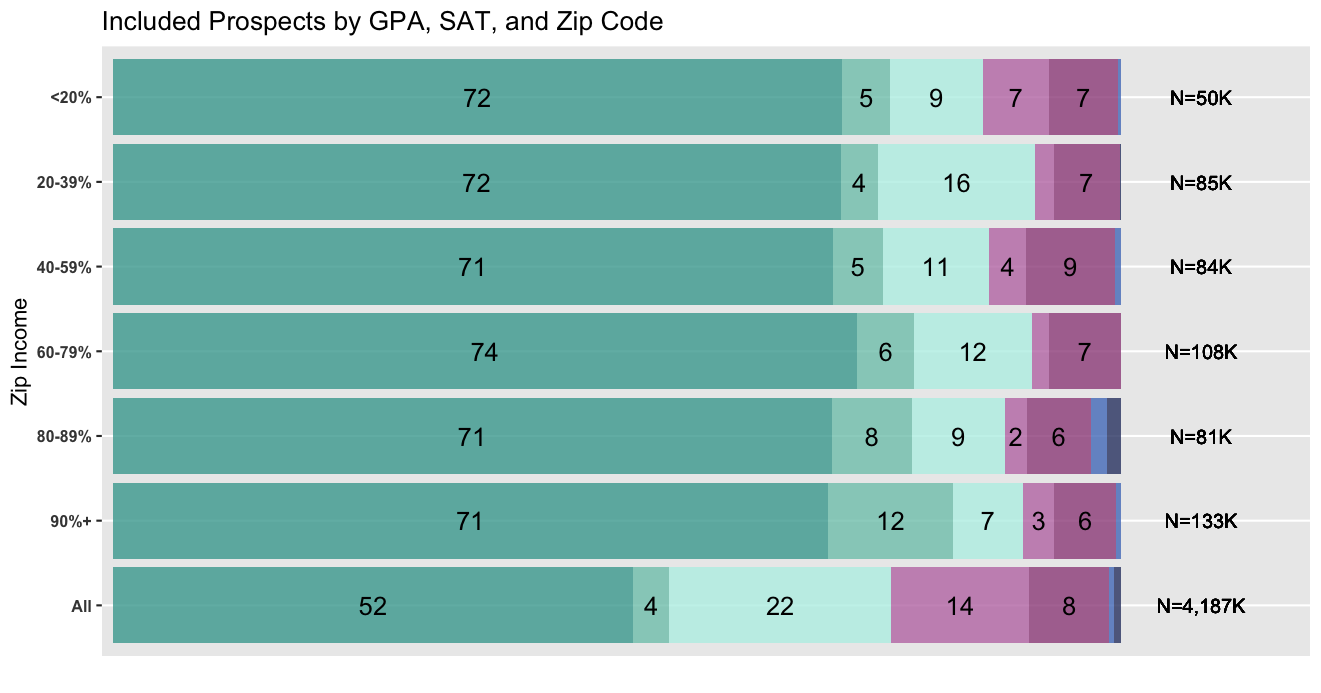
\includegraphics[width=0.35\linewidth]{./../../outputs/figures/combo2_inc_satV2} 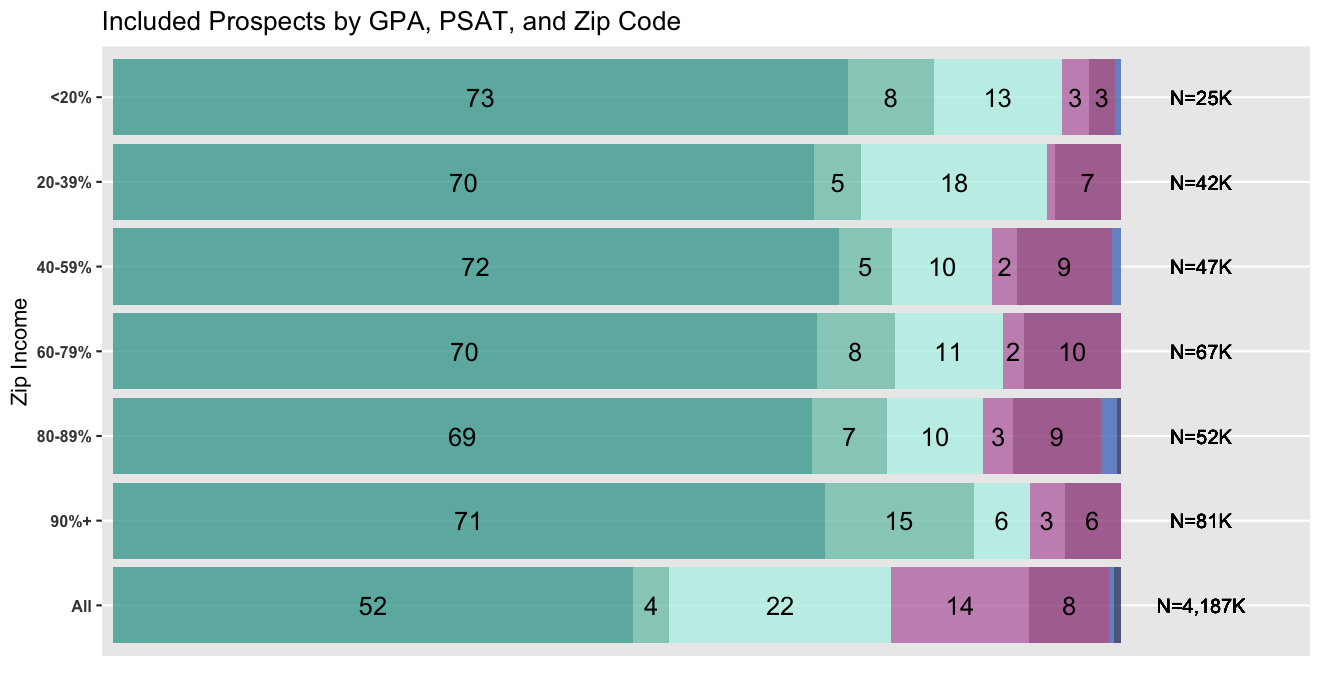
\includegraphics[width=0.35\linewidth]{./../../outputs/figures/combo2_inc_psatV2} 

}

\caption{Academic and Geographic Combination: GPA (3.0+), College Pre-Entrance (150+) or Entrance (1050+) Exams, and Zip (across income thresholds)}\label{fig:gpa-sat-psat-zip}
\end{figure}


\begin{center}
\includegraphics[width=0.32\linewidth]{./../../outputs/figures/legend_horizontal} \end{center}

\begingroup
\fontsize{8}{8}\selectfont
SOURCE: U.S. Department of Education, National Center for Education Statistics, High School Longitudinal Study of 2009 (HSLS09).
\endgroup

\end{landscape}

\restoregeometry

\clearpage

\begin{figure}
\centering
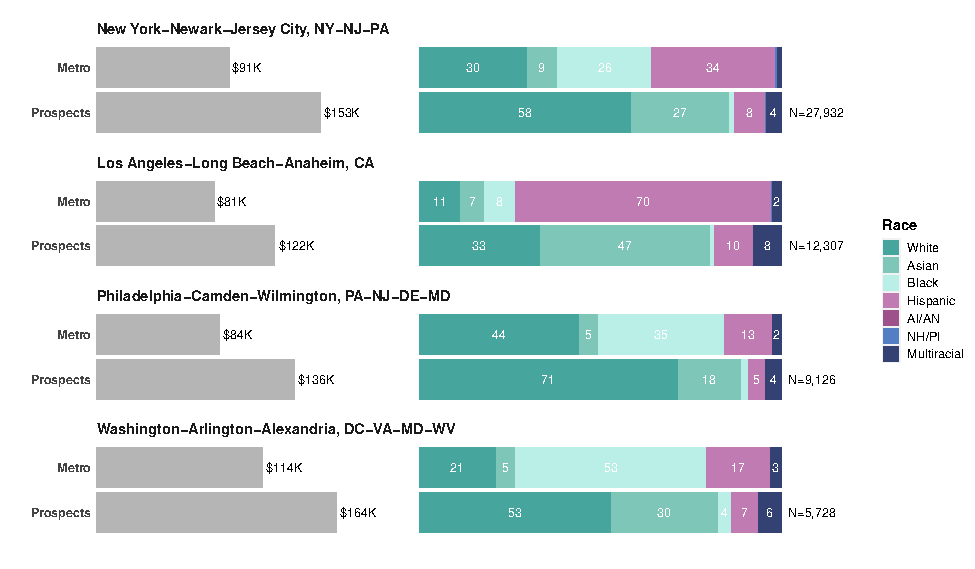
\includegraphics{eepa_student_list_manuscript_c_a_files/figure-latex/uiuc-deep-dive-1.pdf}
\caption{\label{fig:uiuc-deep-dive}Segment Filter Prospects by Metropolitan Area}
\end{figure}

\begingroup
\fontsize{10}{10}\selectfont

\emph{Note: Filters used across these orders include HS Class, GPA (B-A+), State (in-state vs.~out-of-state), AP STEM (3 min for in-state; 4 min for out-of-state) or SAT (1200 minimum for in-state; 1300 minimum for out-of-state) with STEM major interest. Metro population source is the National Center for Education Statistic's Common Core of Data and includes all students attending a public high school in the metropolitan area. }
\endgroup

\pagebreak

\begin{landscape}

\begin{figure}

{\centering 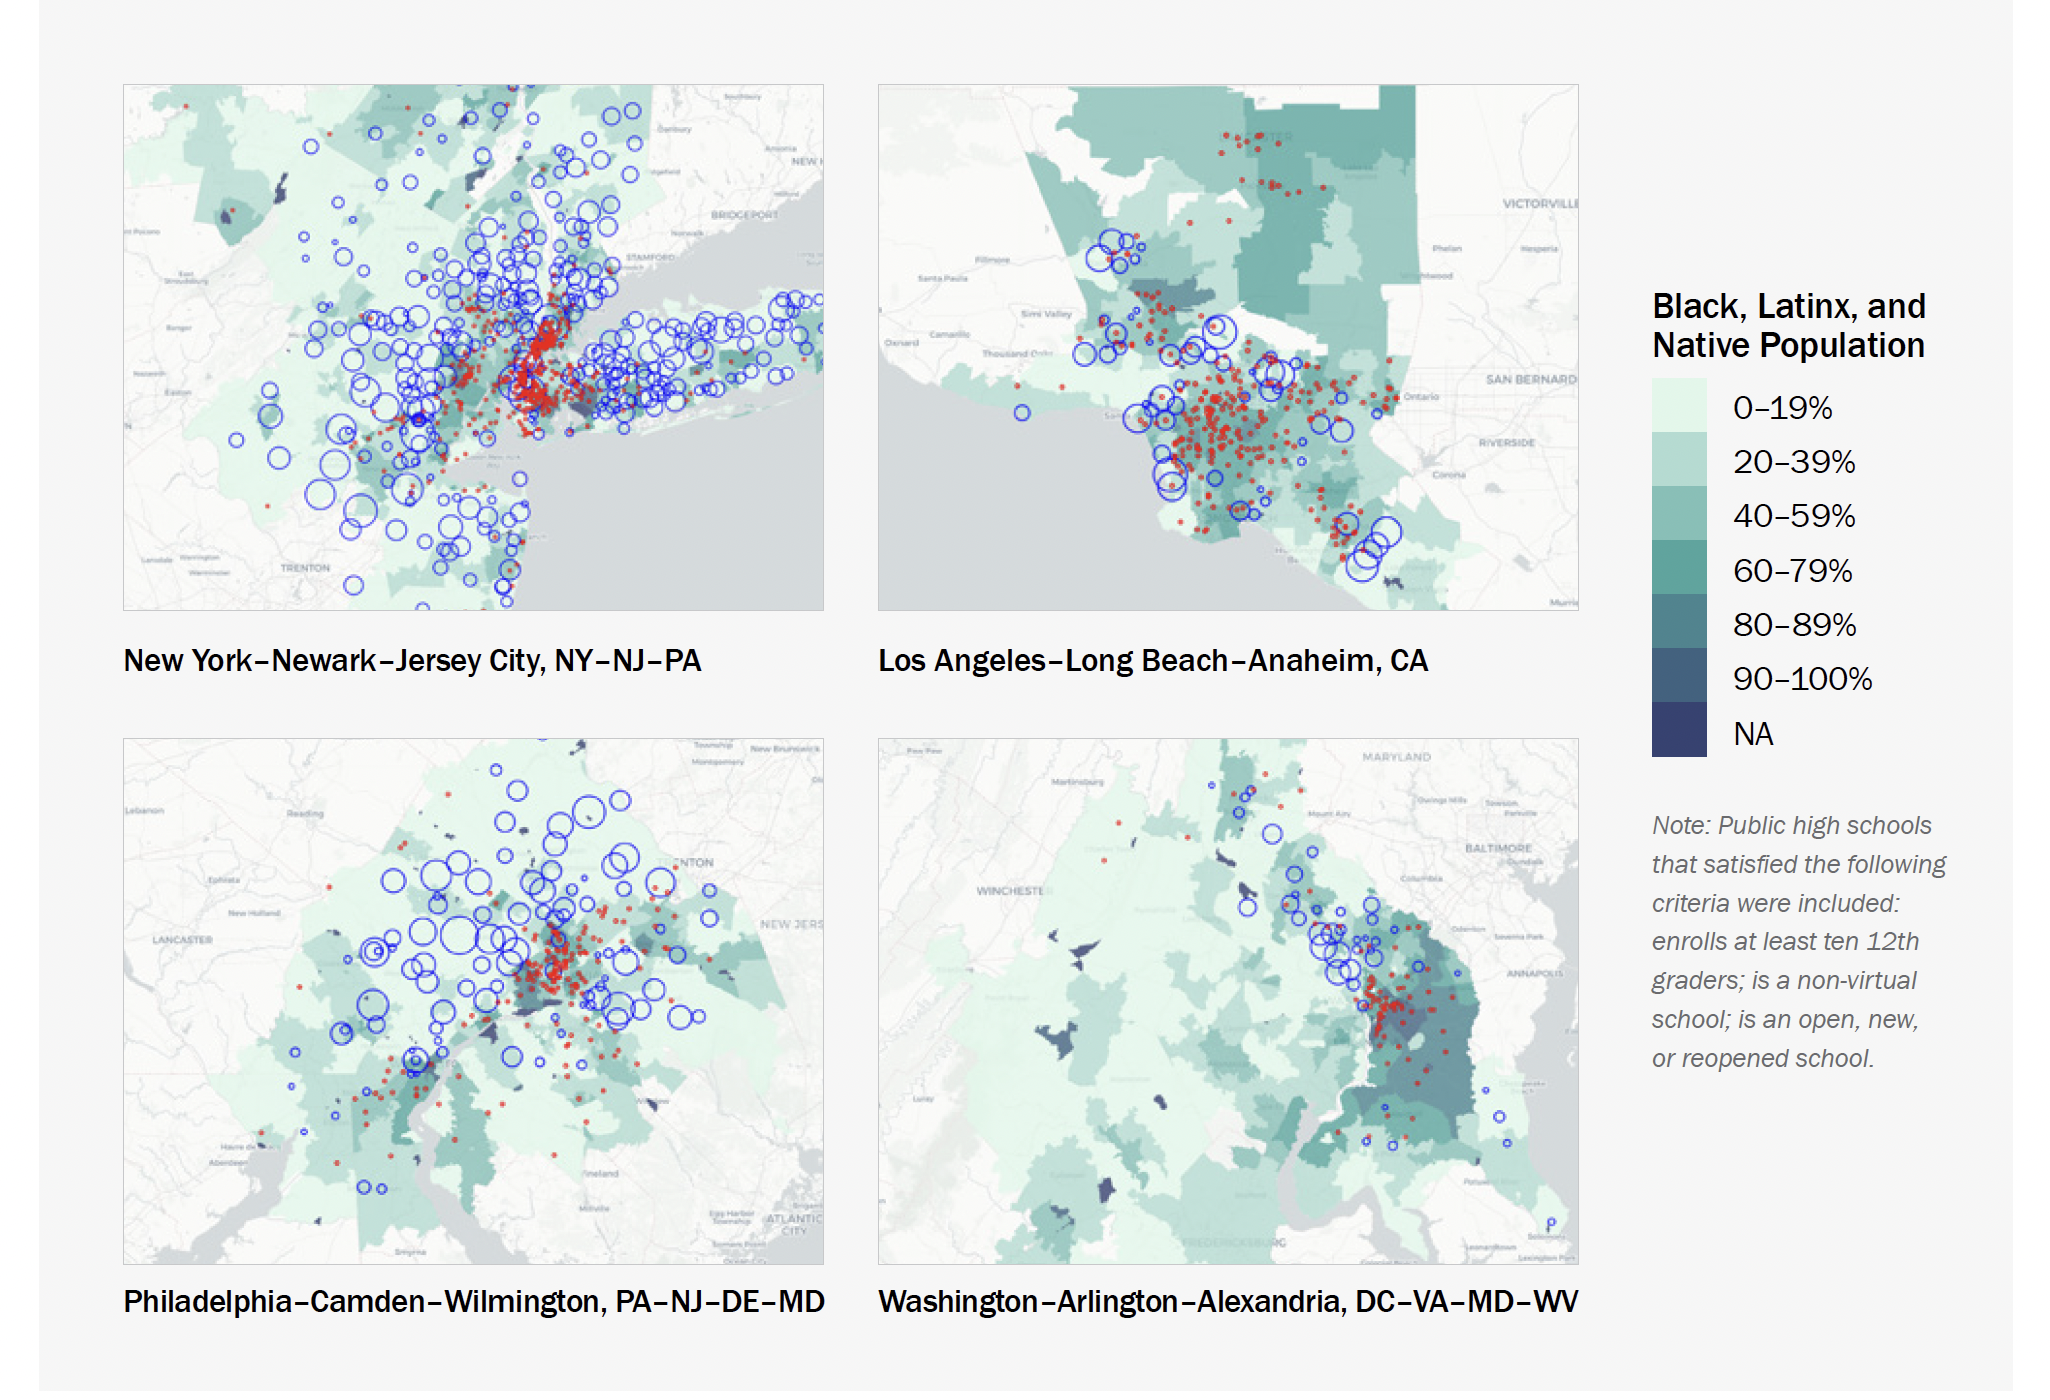
\includegraphics[width=1\linewidth]{./../../outputs/images/uiuc-map} 

}

\caption{Maps of Segment Filter Prospects by Metropolitan Area}\label{fig:uiuc-map}
\end{figure}

\end{landscape}

\pagebreak

\clearpage

\begin{figure}
\centering
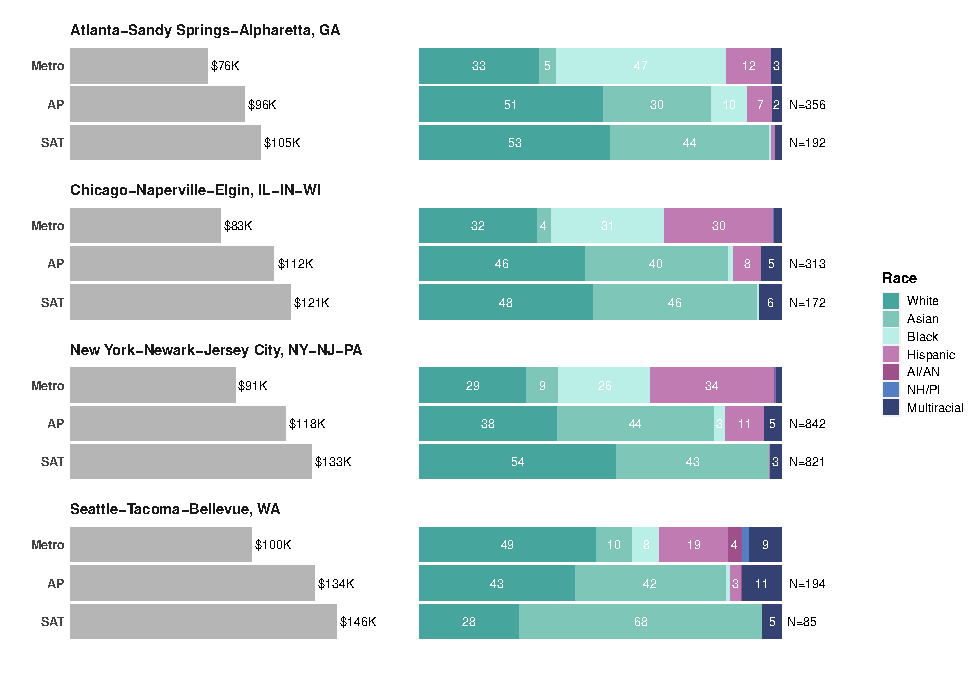
\includegraphics{eepa_student_list_manuscript_c_a_files/figure-latex/ucsd-deep-dive-1.pdf}
\caption{\label{fig:ucsd-deep-dive}Women in STEM Prospects by Metropolitan Area}
\end{figure}

\begingroup
\fontsize{10}{10}\selectfont

\emph{Note: Filters used across these orders include HS Class, Segment, GPA (B-A+), PSAT/SAT (1220-1450); State/CBSAs. Metro population source is the National Center for Education Statistic's Common Core of Data and includes all students attending a public high school in the metropolitan area. }
\endgroup

\end{document}
